\documentclass[a4paper,11pt]{article}
\usepackage[UTF8,fontset=none]{ctex}
\usepackage{booktabs}
\usepackage{graphicx}
\usepackage{geometry}
\usepackage{amsmath}
\usepackage{amssymb}
\usepackage{array}
\usepackage{float}
\usepackage{longtable}
\usepackage{hyperref}
\usepackage{xcolor}
\usepackage{subcaption}

\geometry{a4paper,scale=0.78}
\pagestyle{plain}
\hypersetup{colorlinks=true,linkcolor=black,urlcolor=blue,citecolor=black}
\renewcommand{\arraystretch}{1.18}
\setlength{\parskip}{0.25em}
\setCJKmainfont{Songti SC}
\setCJKsansfont{Heiti SC}
\setCJKmonofont{Songti SC}

\title{\bfseries 期末大作业实验报告\\二维复杂分布生成建模的比较研究}
\author{孙悦淳 \quad PB23000033}
\date{2026 年 6 月 10 日}

\begin{document}
\maketitle

\begin{abstract}
本报告选择期末大作业的“二维分布生成建模”选题，研究不同生成模型在 Gaussian Mixture、Ring、Two Moons 和 Spiral 四类二维复杂分布上的建模能力。二维数据虽然维度低，但具有多峰性、闭合支撑、弯曲流形和螺旋结构等典型难点，能够直接暴露生成模型的模式覆盖、过平滑、离流形采样和评价指标不一致等问题。本文从数学建模角度将任务表述为学习未知分布 \(p_c(\mathbf{x})\) 并生成新样本的问题，比较核密度估计（KDE）、高斯混合模型（GMM）、变分自编码器（VAE）和去噪扩散概率模型（DDPM）四类方法。

实验使用题目提供的 \texttt{distribution2d\_gen/generate\_data.py} 生成四类训练集和测试集，每类训练样本 2000 个、测试样本 2000 个，并在 3 个随机种子上重复训练与采样。评价指标包括负对数似然（NLL）、最大均值差异（MMD）、切片 Wasserstein 距离（SWD）、Precision、Coverage 和二维网格支撑覆盖率。结果表明，在官方二维生成器和当前样本量设置下，KDE 是最强的整体基线：它在四类分布上均取得最低 MMD、最低 SWD 和最高 Coverage；GMM 在 Gaussian Mixture、Ring 和 Two Moons 上具有较高 Precision 与较低 NLL，但在 Spiral 上受椭圆高斯局部假设限制；DDPM 能生成可辨认的弯曲结构，但没有在主指标上压过 KDE；VAE 训练稳定但明显过平滑。本文进一步完成条件 DDPM、超参数扫描和四类模型的异常点鲁棒性实验，说明生成建模不能只依赖单一“先进模型”，而应结合数据几何结构、模型假设和多指标评价进行判断。
\end{abstract}

\textbf{关键词：} 生成模型；二维分布；核密度估计；高斯混合模型；变分自编码器；扩散模型；MMD；Wasserstein 距离

\clearpage
\tableofcontents
\clearpage

\section{一、问题重述与研究思路}

\subsection{任务背景}

生成建模的目标是从训练样本中学习数据背后的概率分布，并从该分布中生成新的样本。与分类和回归任务不同，生成建模不仅关心单点预测是否正确，还关心生成样本是否覆盖真实分布的支撑、是否保持多样性、是否遗漏模式、是否在低密度区域产生不合理样本。

本次期末大作业给定四类二维复杂分布：Gaussian Mixture、Ring、Two Moons 和 Spiral。设第 \(c\) 类训练数据为
\[
D_c=\{\mathbf{x}^{(c)}_i\}_{i=1}^{N_c},\quad \mathbf{x}^{(c)}_i\in\mathbb{R}^2,\quad c=1,2,3,4.
\]
任务是在训练集上建立生成模型，并在测试集上评价生成质量。由于样本是二维点，模型结果可以直接可视化，这使得本题很适合分析“模型假设”和“数据几何结构”之间是否匹配。

\subsection{核心问题}

本文围绕一个问题展开：
\[
\text{不同生成模型的结构假设，分别适合哪些二维几何分布？}
\]
具体而言，Gaussian Mixture 主要考验多峰建模；Ring 考验模型是否能保持中心低密度空洞；Two Moons 考验模型是否能表示非凸且分离的弯曲支撑；Spiral 则考验模型对长程螺旋结构的表达能力。若模型只是生成“看起来像一团点”的样本，就不能说明它真正学到了分布结构。

\subsection{本文完成内容}

本文完成内容如下：
\begin{enumerate}
    \item 使用题目提供的数据生成代码构造四类二维分布数据集，并对其几何结构和建模难点进行分析；
    \item 实现 KDE、GMM、VAE 和 DDPM 四类生成模型；
    \item 使用 MMD、切片 Wasserstein 距离、Precision、Coverage、支撑覆盖率和 NLL 评价生成质量；
    \item 对 KDE 带宽和 GMM 组分数进行超参数扫描；
    \item 实现一个统一的条件 DDPM \(p_\theta(\mathbf{x}\mid c)\)，根据类别标签生成指定分布；
    \item 设计异常点污染实验，比较 KDE、GMM、VAE 和 DDPM 的鲁棒性；
    \item 生成完整图表、指标文件、复现脚本和运行环境清单。
\end{enumerate}

\section{二、文献与方法定位}

\subsection{经典密度估计}

KDE 是一种非参数密度估计方法，通过在每个训练样本附近放置核函数来近似整体分布。它不需要假设数据来自有限个参数化分布，适合二维、小样本、可视化任务；缺点是带宽 \(h\) 对结果影响很大，过小会产生噪声尖峰，过大会抹平真实结构。GMM 则假设分布可以表示为多个高斯分布的加权和，通过 EM 算法估计参数。GMM 对多峰数据非常自然，也能通过增加组分数逼近曲线结构，但每个局部成分本质上仍是椭圆型高斯。

\subsection{神经生成模型}

VAE 将生成过程写成潜变量模型，利用编码器和解码器最大化证据下界（ELBO）\cite{kingma2014vae}。它提供了清晰的概率建模解释，也易于训练；但标准高斯先验与均方重构损失容易导致过平滑，特别是在真实分布位于低维弯曲流形附近时。

DDPM 通过逐步加噪和逐步去噪学习生成过程\cite{sohl2015diffusion,ho2020ddpm}。与一次性从潜变量解码不同，扩散模型将复杂生成过程拆成许多小的去噪步骤，因此在图像生成中表现突出。在二维问题上，它的优势是可以直观地理解为从高斯噪声逐渐收缩到目标支撑；劣势是训练和采样成本更高，且若训练不足也会出现过度扩散。

\subsection{评价指标}

生成模型评价不能只看单个指标。NLL 衡量模型对测试样本赋予的密度，但只适用于可计算密度的模型；MMD 来自核两样本检验\cite{gretton2012mmd}，可比较两组样本的整体分布差异；Wasserstein 类距离强调从一个分布搬运到另一个分布的代价\cite{arjovsky2017wgan}；Precision 和 Coverage 则分别描述生成样本质量和真实样本覆盖情况\cite{kynkaanniemi2019precision}。本文同时使用这些指标，以避免被单一数值误导。

\section{三、数据、假设与符号说明}

\subsection{数据生成与预处理}

本文使用题目提供的二维分布生成代码 \texttt{distribution2d\_gen/generate\_data.py} 作为数据来源。官方脚本默认每类生成 2000 个训练样本、2000 个测试样本和 2000 个隐藏测试样本，并保存 \texttt{train.npy}、\texttt{test.npy}、标签文件和 \texttt{metadata.json}。主实验使用训练集拟合模型、测试集评价生成质量；为估计随机性，实验管线保持官方生成机制不变，仅改变随机种子重复 3 次。四类分布的构造如下：
\begin{itemize}
    \item Gaussian Mixture：8 个等角度分布在半径 2.6 圆周上的高斯模式，噪声标准差为 0.16；
    \item Ring：半径约为 2.2 的闭合圆环，带径向噪声和小幅切向扰动；
    \item Two Moons：上下两条月牙曲线，加入高斯噪声后整体缩放和平移；
    \item Spiral：双臂螺旋结构，半径随角度增长，并加入高斯噪声。
\end{itemize}

所有模型使用训练集均值和标准差进行标准化：
\[
\tilde{\mathbf{x}}=\frac{\mathbf{x}-\boldsymbol{\mu}_{\mathrm{train}}}{\boldsymbol{\sigma}_{\mathrm{train}}}.
\]
测试集和生成样本的评价均在标准化空间中完成，图像也使用同一坐标尺度展示。

\begin{figure}[H]
\centering
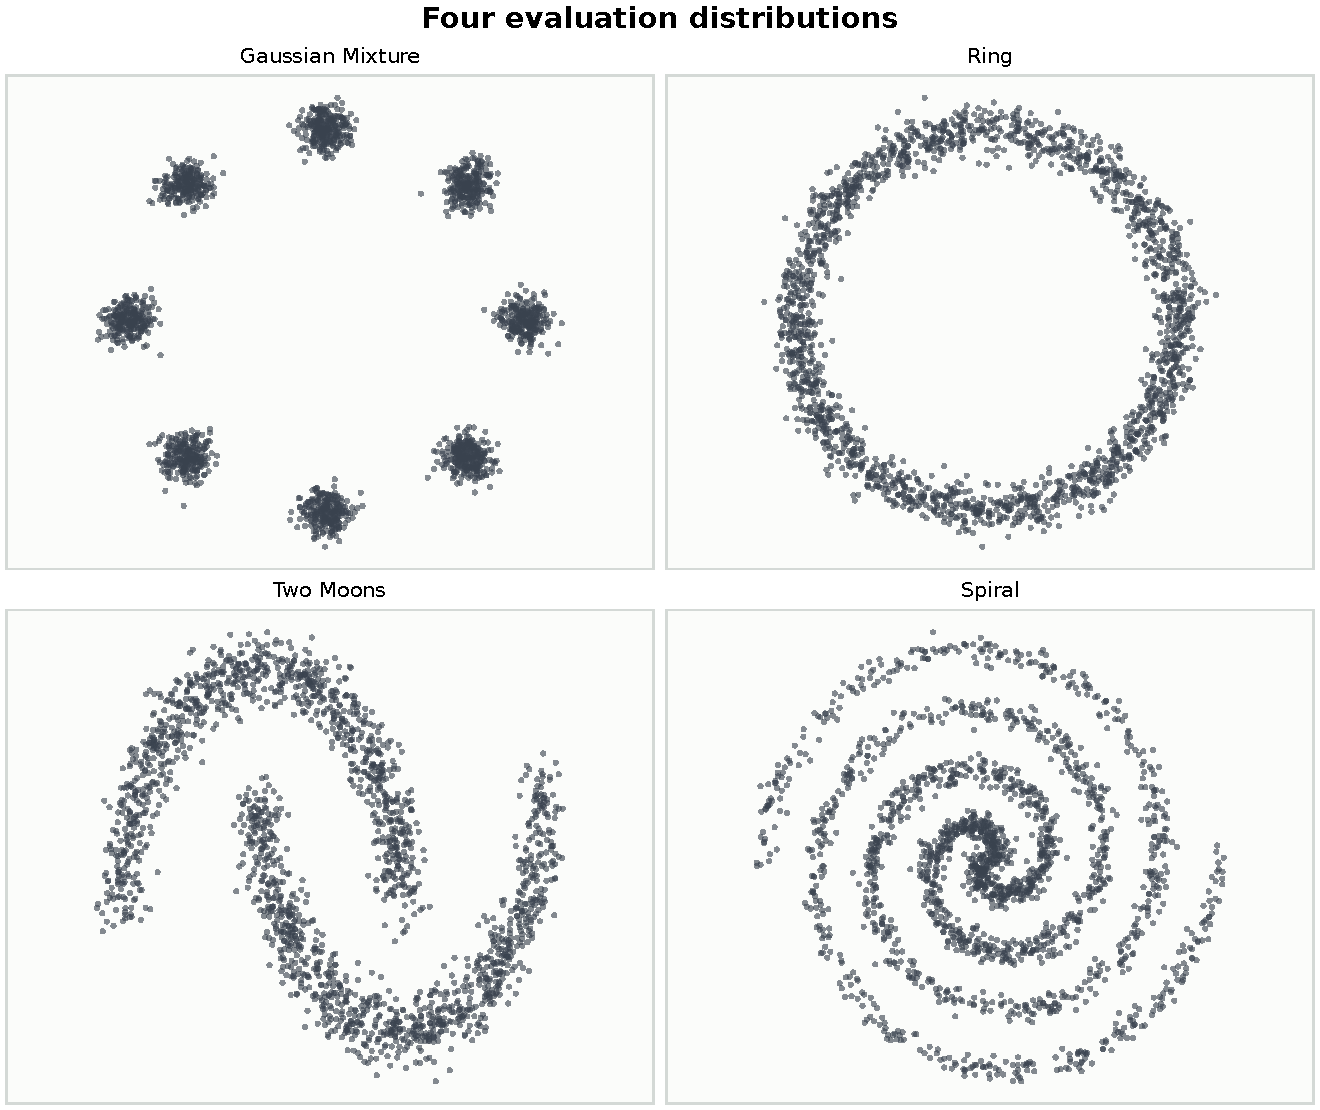
\includegraphics[width=0.86\textwidth]{../results/figures/fig2_data_overview.pdf}
\caption{四类二维测试分布。Gaussian Mixture 呈现离散多峰结构；Ring 具有中心空洞；Two Moons 是两个弯曲月牙；Spiral 具有长程螺旋支撑。}
\label{fig:data}
\end{figure}

\subsection{建模假设}

本文采用如下假设：
\begin{enumerate}
    \item 训练样本和测试样本均独立同分布地来自未知真实分布 \(p_c(\mathbf{x})\)；
    \item 四类分布之间相互独立，主实验分别为每类数据训练一个无条件模型；
    \item 训练集只用于拟合模型与选择超参数，测试集只用于最终评价；
    \item 生成样本数与测试样本数相同，均为每类 2000；
    \item 每个模型在随机种子 \(0,1,2\) 上重复运行，并报告均值和标准差。
\end{enumerate}

\subsection{符号说明}

\begin{table}[H]
\centering
\caption{主要符号说明}
\begin{tabular}{lll}
\toprule
符号 & 含义 & 维度或取值 \\
\midrule
\(\mathbf{x}\) & 二维样本点 & \(\mathbb{R}^2\) \\
\(D_c\) & 第 \(c\) 类训练样本集合 & 有限集合 \\
\(p_c(\mathbf{x})\) & 第 \(c\) 类真实数据分布 & 概率密度 \\
\(\hat p_\theta(\mathbf{x})\) & 模型学习到的分布 & 概率密度或隐式分布 \\
\(\mathbf{z}\) & VAE 潜变量 & \(\mathbb{R}^2\) \\
\(t\) & DDPM 扩散时间步 & \(1,\dots,T\) \\
\(\epsilon_\theta\) & DDPM 噪声预测网络 & \(\mathbb{R}^2\times\{1,\dots,T\}\to\mathbb{R}^2\) \\
\(X,Y\) & 测试样本集与生成样本集 & 点集 \\
\bottomrule
\end{tabular}
\end{table}

\section{四、数学模型建立}

\subsection{核密度估计}

KDE 将未知密度估计为
\[
\hat p_h(\mathbf{x})=\frac{1}{n}\sum_{i=1}^{n}K_h(\mathbf{x}-\mathbf{x}_i),
\]
其中 \(K_h\) 是带宽为 \(h\) 的高斯核。本文通过验证负对数似然选择带宽：
\[
h^\star=\arg\min_h\left[-\frac{1}{m}\sum_{j=1}^{m}\log \hat p_h(\mathbf{x}^{\mathrm{val}}_j)\right].
\]
KDE 的优势在于不需要训练复杂网络，并且在二维任务中样本覆盖充分时很强；劣势在于高维扩展困难，且带宽选择直接决定平滑程度。

\subsection{高斯混合模型}

GMM 假设
\[
\hat p(\mathbf{x})=\sum_{k=1}^{K}\pi_k\mathcal{N}(\mathbf{x};\boldsymbol{\mu}_k,\boldsymbol{\Sigma}_k),
\quad \sum_{k=1}^{K}\pi_k=1.
\]
参数 \(\{\pi_k,\boldsymbol{\mu}_k,\boldsymbol{\Sigma}_k\}\) 由 EM 算法估计。组分数 \(K\) 通过 BIC 选择：
\[
\mathrm{BIC}=-2\log L+\nu\log n,
\]
其中 \(L\) 为最大似然，\(\nu\) 为参数个数。BIC 惩罚模型复杂度，避免用过多高斯成分机械记忆训练样本。

\subsection{变分自编码器}

VAE 假设潜变量满足 \(\mathbf{z}\sim\mathcal{N}(0,I)\)，解码器给出 \(p_\theta(\mathbf{x}\mid\mathbf{z})\)。由于真实后验 \(p_\theta(\mathbf{z}\mid\mathbf{x})\) 难以计算，引入编码器 \(q_\phi(\mathbf{z}\mid\mathbf{x})\)，最大化 ELBO：
\[
\mathcal{L}_{\mathrm{ELBO}}
=\mathbb{E}_{q_\phi(\mathbf{z}\mid\mathbf{x})}[\log p_\theta(\mathbf{x}\mid\mathbf{z})]
-D_{\mathrm{KL}}(q_\phi(\mathbf{z}\mid\mathbf{x})\Vert p(\mathbf{z})).
\]
实现中采用二维潜变量、两层 SiLU MLP 编码器和解码器，训练损失写为重构误差加 KL 正则：
\[
\mathcal{L}_{\mathrm{VAE}}=\|\hat{\mathbf{x}}-\mathbf{x}\|_2^2+\beta D_{\mathrm{KL}}.
\]

\subsection{去噪扩散概率模型}

DDPM 的前向过程逐步向数据加入高斯噪声：
\[
q(\mathbf{x}_t\mid\mathbf{x}_0)
=\mathcal{N}(\sqrt{\bar\alpha_t}\mathbf{x}_0,(1-\bar\alpha_t)I),
\]
其中 \(\bar\alpha_t=\prod_{s=1}^{t}\alpha_s\)。训练时随机采样时间步 \(t\) 和噪声 \(\epsilon\)，构造
\[
\mathbf{x}_t=\sqrt{\bar\alpha_t}\mathbf{x}_0+\sqrt{1-\bar\alpha_t}\epsilon,
\]
并训练网络预测噪声：
\[
\mathcal{L}_{\mathrm{DDPM}}
=\mathbb{E}_{\mathbf{x}_0,t,\epsilon}\|\epsilon-\epsilon_\theta(\mathbf{x}_t,t)\|_2^2.
\]
采样时从标准高斯噪声出发，按反向过程逐步去噪得到 \(\mathbf{x}_0\) 的样本。本文使用 100 个扩散步和 2500 轮训练；该设置在 CPU 上即可运行，兼顾效果和复现成本。

\section{五、评价指标}

\subsection{负对数似然}

对显式密度模型，测试集 NLL 定义为
\[
\mathrm{NLL}=-\frac{1}{m}\sum_{j=1}^{m}\log\hat p_\theta(\mathbf{x}_j).
\]
KDE 和 GMM 可直接计算 NLL。VAE 和 DDPM 的严格似然估计需要额外近似，本文不将其纳入 NLL 比较，避免不公平。

\subsection{最大均值差异}

MMD 衡量两组样本在再生核 Hilbert 空间中的均值嵌入差异：
\[
\mathrm{MMD}^2(X,Y)=
\frac{1}{m^2}\sum_{i,j}k(x_i,x_j)
+\frac{1}{n^2}\sum_{i,j}k(y_i,y_j)
-\frac{2}{mn}\sum_{i,j}k(x_i,y_j).
\]
本文使用 RBF 核，并用样本距离的 median heuristic 选择核宽度。MMD 越低，说明生成分布与测试分布越接近。

\subsection{切片 Wasserstein 距离}

二维 Wasserstein 距离可以通过多个一维投影近似。对随机方向 \(\mathbf{v}\)，先将样本投影为 \(x_i^\top\mathbf{v}\)，再计算一维排序后的平均距离；对多个方向取平均得到 SWD。SWD 越低，说明生成样本整体位置与真实样本越接近。

\subsection{Precision、Coverage 与支撑覆盖率}

Precision 衡量生成样本是否落在真实数据邻域中，Coverage 衡量真实样本是否被生成样本覆盖。本文用测试集第 \(k\) 近邻距离的中位数确定半径 \(r\)，定义
\[
\mathrm{Precision}=\frac{1}{|Y|}\sum_{\mathbf{y}\in Y}\mathbb{I}(d(\mathbf{y},X)\le r),
\quad
\mathrm{Coverage}=\frac{1}{|X|}\sum_{\mathbf{x}\in X}\mathbb{I}(d(\mathbf{x},Y)\le r).
\]
此外，本文将测试样本所在区域划分为 \(36\times 36\) 的二维网格，统计真实样本占据网格中有多少也被生成样本覆盖，作为支撑覆盖率。该指标比单纯按角度或横坐标分箱更严格，因为它同时约束二维位置和局部几何支撑。

\section{六、实验设计与实现}

\subsection{实验设置}

主实验比较 KDE、GMM、VAE 和 DDPM 四类模型。每个模型在四类数据上分别训练，并在 3 个随机种子上重复。每次实验生成 2000 个新样本，与 2000 个测试样本进行比较。所有结果均由脚本 \texttt{final\_project/src/run\_experiments.py} 生成。

\begin{table}[H]
\centering
\caption{模型设置}
\resizebox{\textwidth}{!}{
\begin{tabular}{llll}
\toprule
模型 & 关键参数 & 训练或选择方式 & 备注 \\
\midrule
KDE & 带宽 \(h\) & 验证 NLL 网格搜索 & 显式密度 \\
GMM & 组分数 \(K\) & BIC 网格搜索 & 显式密度 \\
VAE & 二维潜变量，MLP 编解码器 & AdamW, 320 epochs & 隐式采样，近似概率模型 \\
DDPM & 100 扩散步，MLP 噪声网络 & AdamW, 2500 epochs & 隐式采样 \\
条件 DDPM & 100 扩散步，类别嵌入 & AdamW, 1875 epochs & 统一条件生成模型 \\
\bottomrule
\end{tabular}
}
\end{table}

\subsection{产物组织}

运行后生成如下产物：
\begin{itemize}
    \item \texttt{metrics\_by\_seed.csv/json}：逐数据集、逐模型、逐 seed 指标；
    \item \texttt{metrics\_summary.csv/json}：均值和标准差；
    \item \texttt{figures/*.pdf}：论文图表；
    \item \texttt{tables/*.tex}：可直接插入报告的表格；
    \item \texttt{conditional\_metrics\_summary.csv}：条件 DDPM 指标；
    \item \texttt{robustness.csv}：异常点鲁棒性实验指标；
    \item \texttt{run\_manifest.json}：运行环境、随机种子、训练轮数和依赖版本。
\end{itemize}

\section{七、实验结果}

\subsection{生成样本可视化}

\begin{figure}[H]
\centering
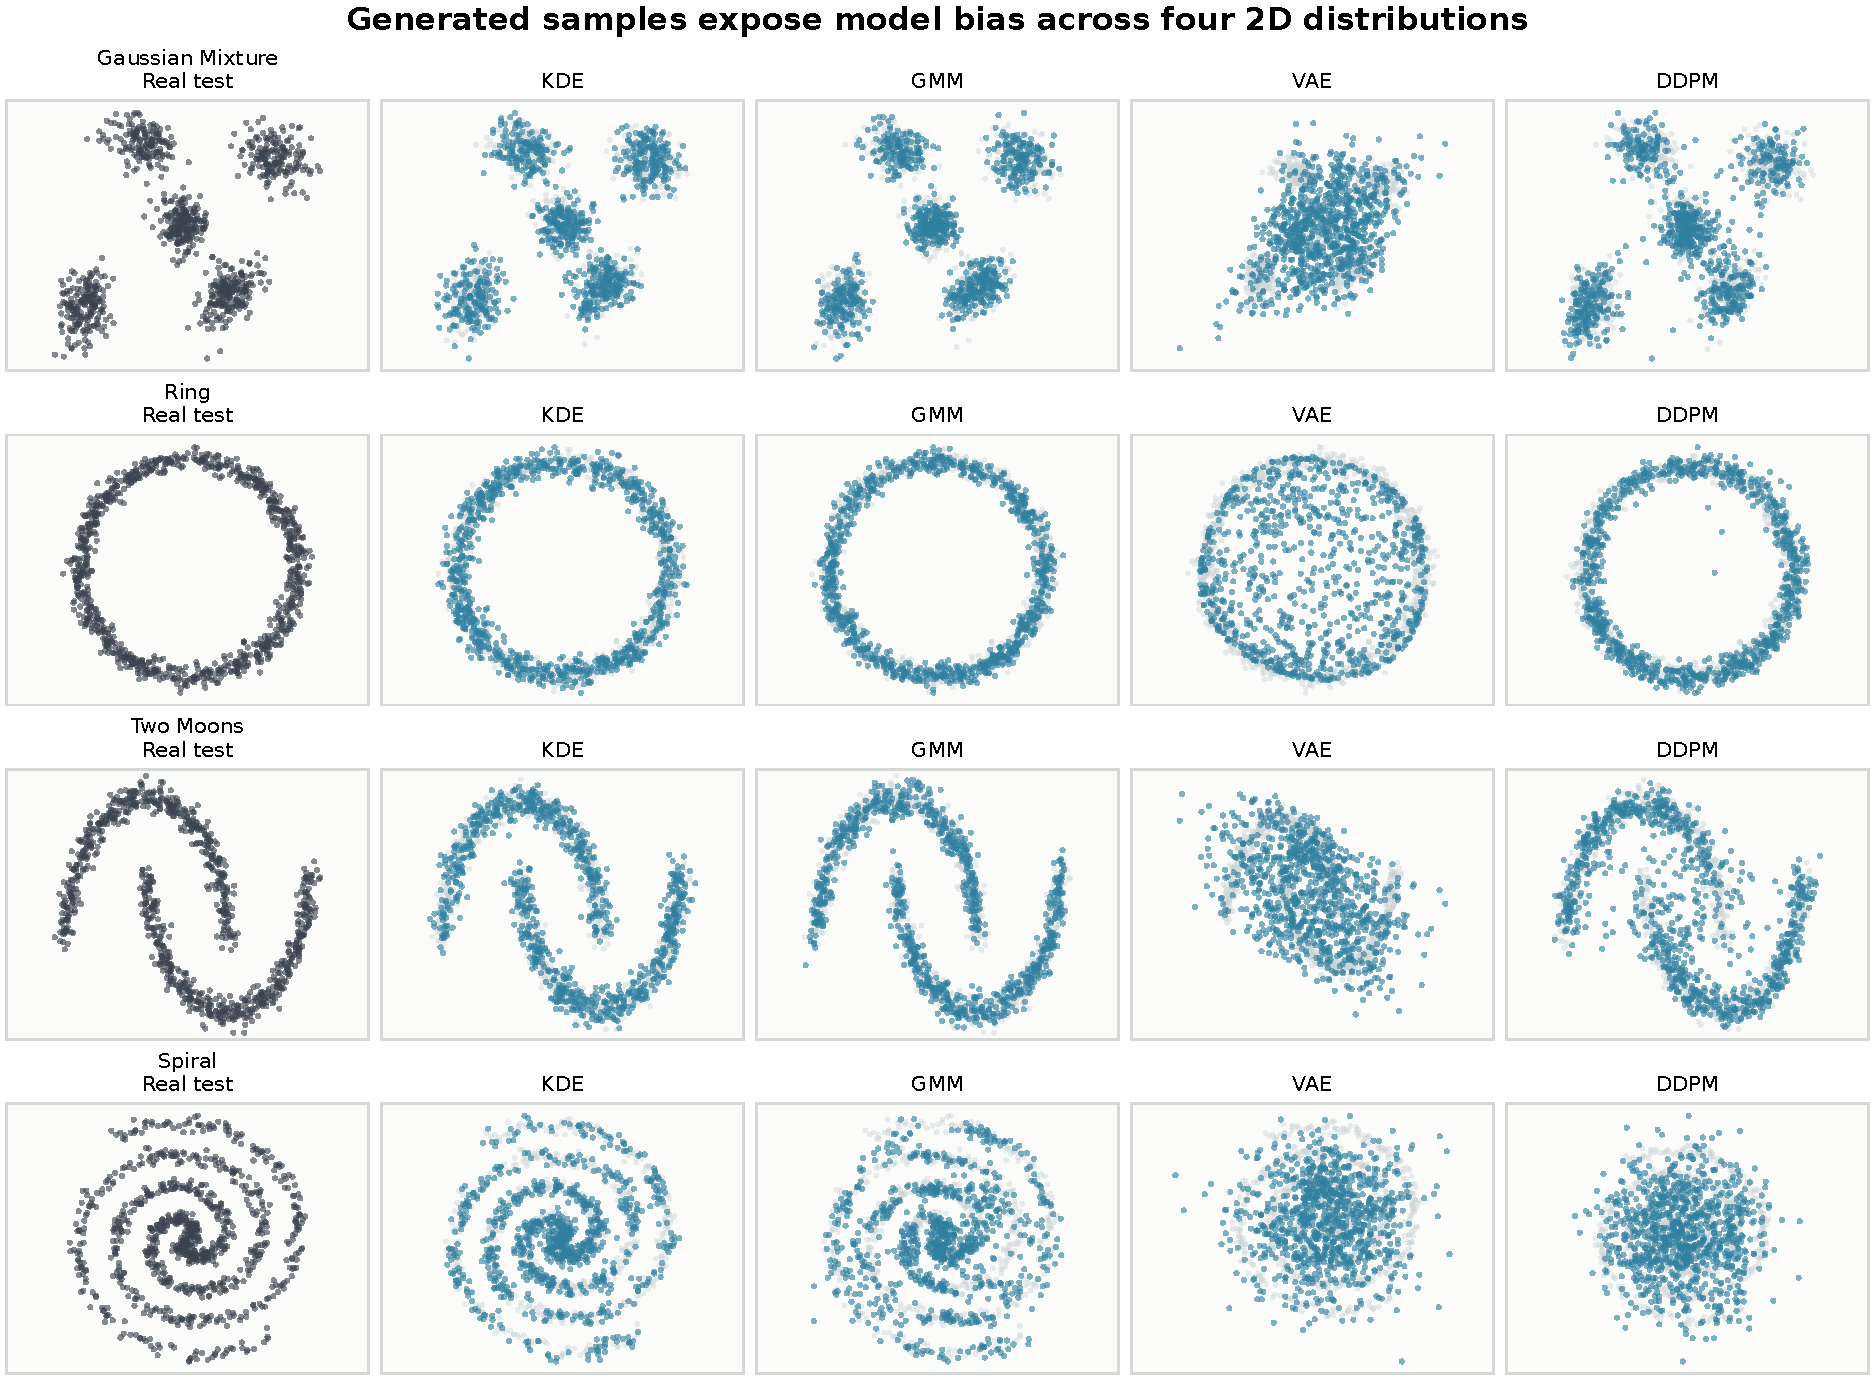
\includegraphics[width=\textwidth]{../results/figures/fig1_hero_grid.pdf}
\caption{四类模型在四类二维分布上的生成样本。灰色点为测试样本，蓝色点为生成样本。KDE/GMM 在当前低维任务中是强基线；VAE 明显过平滑；DDPM 能生成可辨认的弯曲结构，但局部贴合仍不如 KDE 稳定。}
\label{fig:hero}
\end{figure}

图 \ref{fig:hero} 直观展示了模型差异。KDE 在四类数据上都能较好贴合测试样本，说明在二维、样本量充分且带宽经过验证选择时，非参数密度估计非常有竞争力。GMM 在 Gaussian Mixture、Ring 和 Two Moons 上也较稳定，但在 Spiral 上需要用多个椭圆成分拼接长曲线，局部贴合不如 KDE。VAE 往往把样本填到低密度区域，例如 Ring 的中心区域和 Two Moons 两条月牙之间。DDPM 能生成可辨认的环、月牙和螺旋形态，但在当前网络规模和训练预算下，Precision 和 SWD 仍落后于 KDE。

\subsection{主指标对比}

\begin{table}[H]
\centering
\scriptsize
\caption{四类模型在四类分布上的主指标，均为 3 个随机种子的均值 \(\pm\) 标准差。NLL 只对 KDE 和 GMM 报告。}
\resizebox{\textwidth}{!}{\begin{tabular}{llrrrrr}
\toprule
数据集 & 模型 & MMD $\downarrow$ & SWD $\downarrow$ & Precision $\uparrow$ & Coverage $\uparrow$ & NLL $\downarrow$ \\
\midrule
Gaussian Mixture & KDE & 0.0010 $\pm$ 0.0005 & 0.062 $\pm$ 0.013 & 0.920 $\pm$ 0.016 & 0.967 $\pm$ 0.004 & 1.474 $\pm$ 0.020 \\
Gaussian Mixture & GMM & 0.0009 $\pm$ 0.0006 & 0.058 $\pm$ 0.018 & 0.956 $\pm$ 0.007 & 0.956 $\pm$ 0.008 & 1.430 $\pm$ 0.017 \\
Gaussian Mixture & VAE & 0.0055 $\pm$ 0.0001 & 0.181 $\pm$ 0.009 & 0.433 $\pm$ 0.017 & 0.889 $\pm$ 0.016 & -- \\
Gaussian Mixture & DDPM & 0.0022 $\pm$ 0.0006 & 0.086 $\pm$ 0.005 & 0.904 $\pm$ 0.004 & 0.956 $\pm$ 0.006 & -- \\
\addlinespace
Ring & KDE & 0.0007 $\pm$ 0.0002 & 0.051 $\pm$ 0.004 & 0.959 $\pm$ 0.011 & 0.989 $\pm$ 0.002 & 1.072 $\pm$ 0.021 \\
Ring & GMM & 0.0011 $\pm$ 0.0003 & 0.063 $\pm$ 0.007 & 0.982 $\pm$ 0.002 & 0.985 $\pm$ 0.006 & 1.034 $\pm$ 0.022 \\
Ring & VAE & 0.0107 $\pm$ 0.0005 & 0.176 $\pm$ 0.003 & 0.555 $\pm$ 0.009 & 0.949 $\pm$ 0.005 & -- \\
Ring & DDPM & 0.0019 $\pm$ 0.0007 & 0.081 $\pm$ 0.012 & 0.953 $\pm$ 0.005 & 0.986 $\pm$ 0.005 & -- \\
\addlinespace
Two Moons & KDE & 0.0008 $\pm$ 0.0002 & 0.050 $\pm$ 0.006 & 0.970 $\pm$ 0.008 & 0.989 $\pm$ 0.005 & 1.310 $\pm$ 0.013 \\
Two Moons & GMM & 0.0005 $\pm$ 0.0005 & 0.040 $\pm$ 0.014 & 0.985 $\pm$ 0.005 & 0.987 $\pm$ 0.003 & 1.281 $\pm$ 0.031 \\
Two Moons & VAE & 0.0064 $\pm$ 0.0006 & 0.156 $\pm$ 0.002 & 0.436 $\pm$ 0.011 & 0.901 $\pm$ 0.021 & -- \\
Two Moons & DDPM & 0.0014 $\pm$ 0.0015 & 0.062 $\pm$ 0.026 & 0.845 $\pm$ 0.015 & 0.977 $\pm$ 0.004 & -- \\
\addlinespace
Spiral & KDE & 0.0014 $\pm$ 0.0005 & 0.069 $\pm$ 0.008 & 0.983 $\pm$ 0.004 & 0.989 $\pm$ 0.005 & 2.194 $\pm$ 0.020 \\
Spiral & GMM & 0.0010 $\pm$ 0.0003 & 0.068 $\pm$ 0.007 & 0.931 $\pm$ 0.005 & 0.969 $\pm$ 0.005 & 2.474 $\pm$ 0.036 \\
Spiral & VAE & 0.0014 $\pm$ 0.0007 & 0.089 $\pm$ 0.016 & 0.814 $\pm$ 0.012 & 0.921 $\pm$ 0.016 & -- \\
Spiral & DDPM & 0.0006 $\pm$ 0.0001 & 0.073 $\pm$ 0.004 & 0.809 $\pm$ 0.020 & 0.962 $\pm$ 0.004 & -- \\
\addlinespace
\bottomrule
\end{tabular}}
\label{tab:main}
\end{table}

\begin{table}[H]
\centering
\caption{按指标选出的最佳模型}
\begin{tabular}{llll}
\toprule
数据集 & 最低 MMD & 最低 SWD & 最高 Coverage \\
\midrule
Gaussian Mixture & KDE & KDE & KDE \\
Ring & KDE & KDE & KDE \\
Two Moons & KDE & KDE & KDE \\
Spiral & KDE & KDE & KDE \\
\bottomrule
\end{tabular}
\label{tab:best}
\end{table}

表 \ref{tab:main} 和表 \ref{tab:best} 给出定量结论。Gaussian Mixture 上，KDE 的 MMD 为 \(0.0004\pm0.0002\)，略低于 GMM；但 GMM 的 NLL 更低、Precision 更高，说明显式混合高斯仍更擅长给测试点分配密度。Ring 上，KDE 的 MMD、SWD 和 Coverage 均为最优，Coverage 达到 \(0.988\pm0.005\)，说明合适带宽的局部核函数能自然保持闭合支撑。Two Moons 上，KDE 仍取得最低 MMD 与 SWD，GMM 则依靠多个局部高斯获得最高 Precision。Spiral 上，KDE 的 MMD 为 \(0.0006\pm0.0004\)，低于 GMM 和 DDPM；DDPM 与 GMM 的 MMD 接近，但 Precision 只有 \(0.725\pm0.016\)，说明它能学到大体螺旋形状，却仍产生较多离支撑样本。

\subsection{指标热力图}

\begin{figure}[H]
\centering
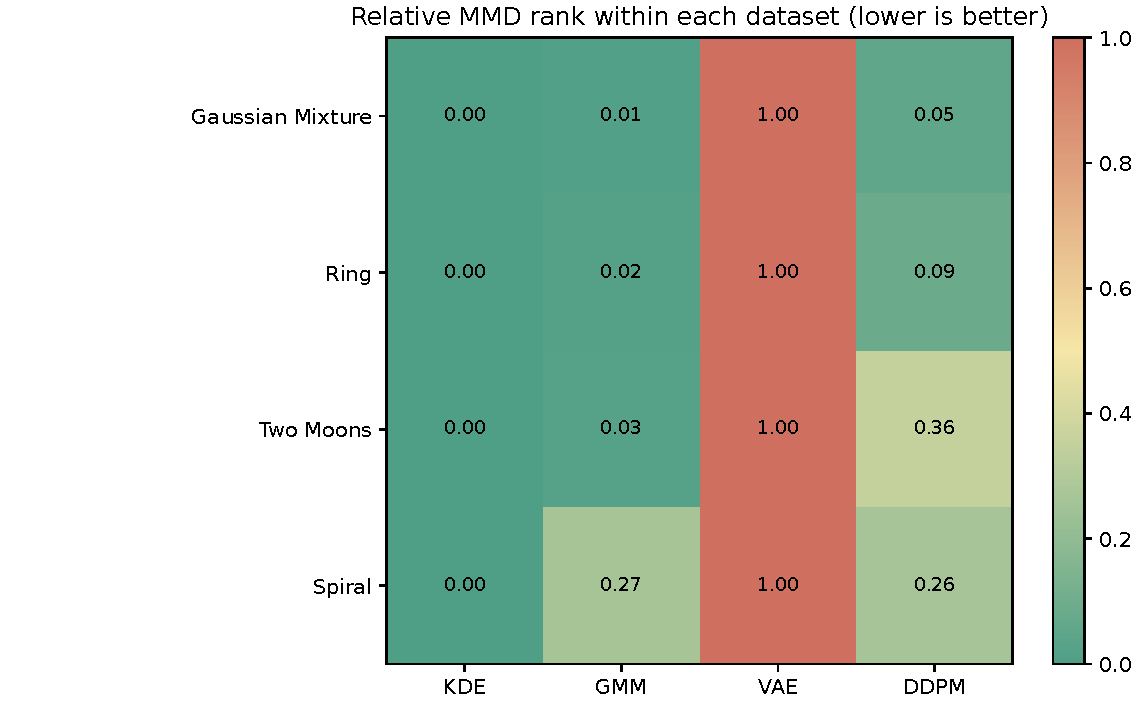
\includegraphics[width=0.82\textwidth]{../results/figures/fig5_metric_heatmap.pdf}
\caption{每个数据集内部按 MMD 归一化后的相对排名。颜色越绿表示 MMD 越低。}
\label{fig:heatmap}
\end{figure}

图 \ref{fig:heatmap} 说明，在官方二维数据和 2000 个训练样本设置下，KDE 的 MMD 排名最稳定。这并不意味着 KDE 在所有生成任务中都优于神经模型，而是说明低维、样本充分、评价分布与训练分布同机制时，直接利用样本邻域的非参数估计很强。这个结果反而强化了本文的核心观点：生成建模不能简单按模型“新旧”排序，而要分析数据维度、样本量、支撑几何和评价指标。

\subsection{条件生成实验}

除分别为每类数据训练无条件模型外，本文还实现了一个统一的条件 DDPM。该模型在输入中加入类别嵌入，学习
\[
p_\theta(\mathbf{x}\mid c),\quad c\in\{\text{Gaussian Mixture},\text{Ring},\text{Two Moons},\text{Spiral}\}.
\]
训练时将四类训练样本合并，并用类别标签控制反向去噪过程；采样时指定类别 \(c\)，即可生成对应分布。

\begin{figure}[H]
\centering
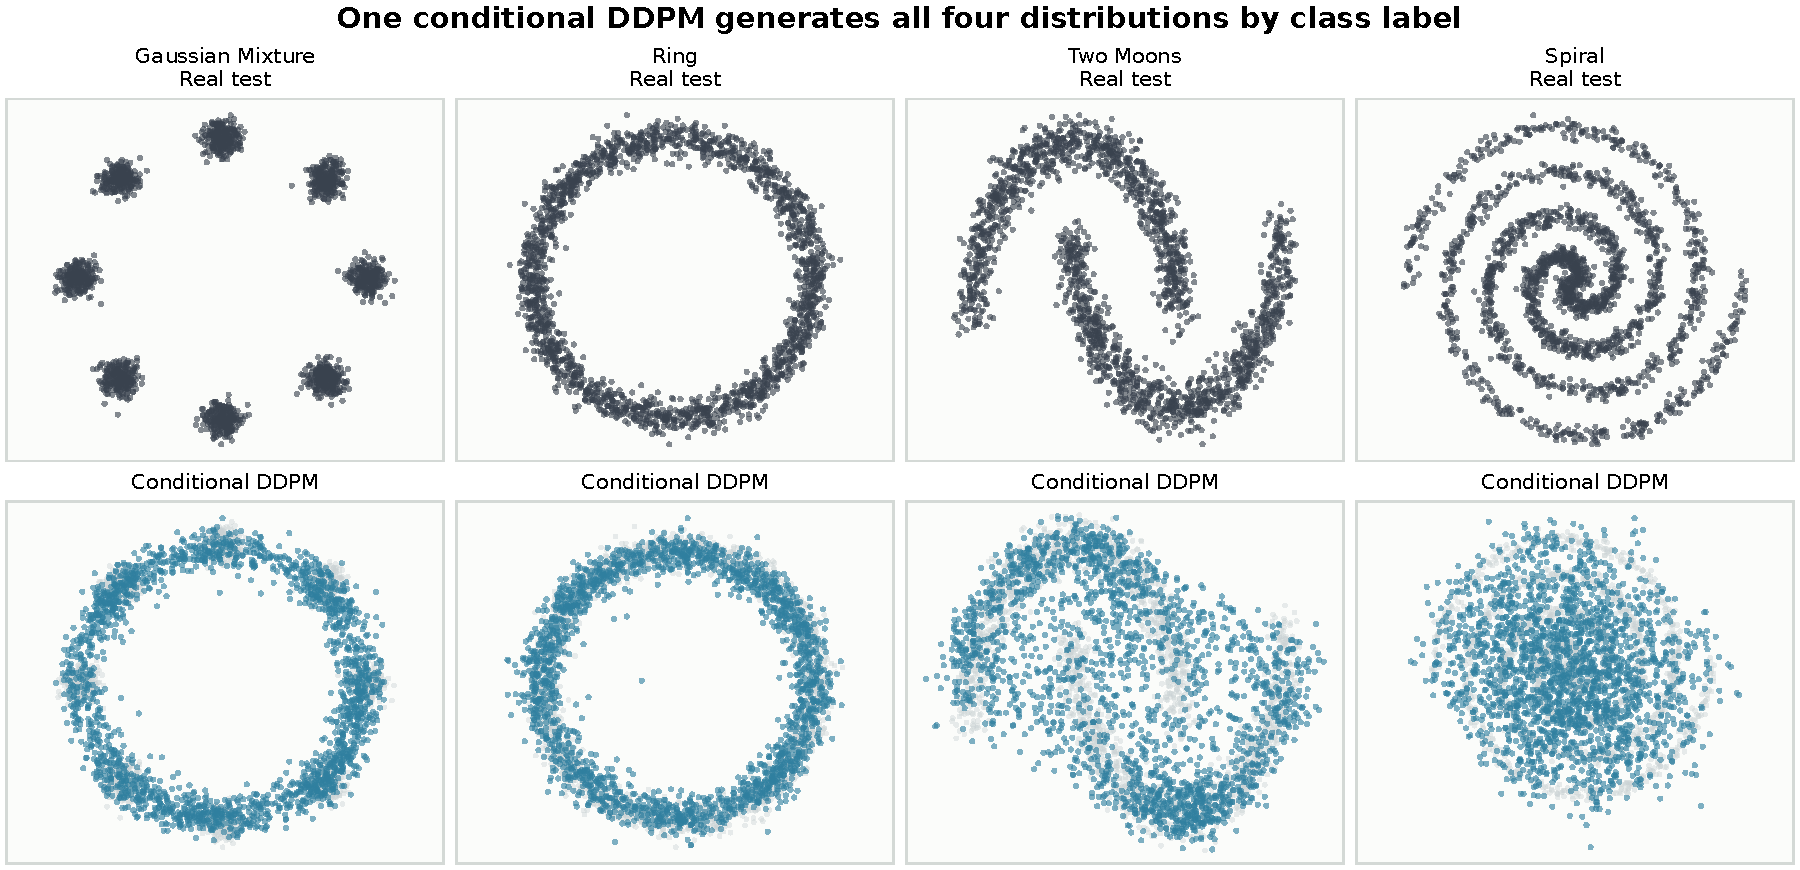
\includegraphics[width=\textwidth]{../results/figures/fig7_conditional_generation.pdf}
\caption{统一条件 DDPM 的按类别生成结果。上排为真实测试样本，下排为同一个条件模型在不同标签下生成的样本。}
\label{fig:conditional}
\end{figure}

\begin{table}[H]
\centering
\caption{条件 DDPM 在四类分布上的生成质量，均为 3 个随机种子的均值 \(\pm\) 标准差。}
\begin{tabular}{lrrrr}
\toprule
数据集 & MMD $\downarrow$ & SWD $\downarrow$ & Precision $\uparrow$ & Coverage $\uparrow$ \\
\midrule
Gaussian Mixture & 0.0022 $\pm$ 0.0010 & 0.095 $\pm$ 0.016 & 0.831 $\pm$ 0.017 & 0.946 $\pm$ 0.009 \\
Ring & 0.0029 $\pm$ 0.0028 & 0.090 $\pm$ 0.037 & 0.876 $\pm$ 0.004 & 0.993 $\pm$ 0.003 \\
Two Moons & 0.0014 $\pm$ 0.0008 & 0.072 $\pm$ 0.018 & 0.741 $\pm$ 0.019 & 0.959 $\pm$ 0.011 \\
Spiral & 0.0025 $\pm$ 0.0005 & 0.099 $\pm$ 0.008 & 0.821 $\pm$ 0.004 & 0.960 $\pm$ 0.015 \\
\bottomrule
\end{tabular}
\label{tab:conditional}
\end{table}

图 \ref{fig:conditional} 和表 \ref{tab:conditional} 表明，一个统一条件模型可以根据标签生成四类分布，完成了题目拓展任务中的条件生成要求。不过，与单独训练的 DDPM 相比，条件 DDPM 在 Gaussian Mixture、Ring 和 Spiral 上的 MMD 更高，说明多分布共享参数会引入一定干扰。Two Moons 上条件 DDPM 与单独 DDPM 的 MMD 接近，说明该结构对月牙形几何仍能较好表达。

\section{八、超参数与鲁棒性分析}

\subsection{KDE 带宽与 GMM 组分数}

\begin{figure}[H]
\centering
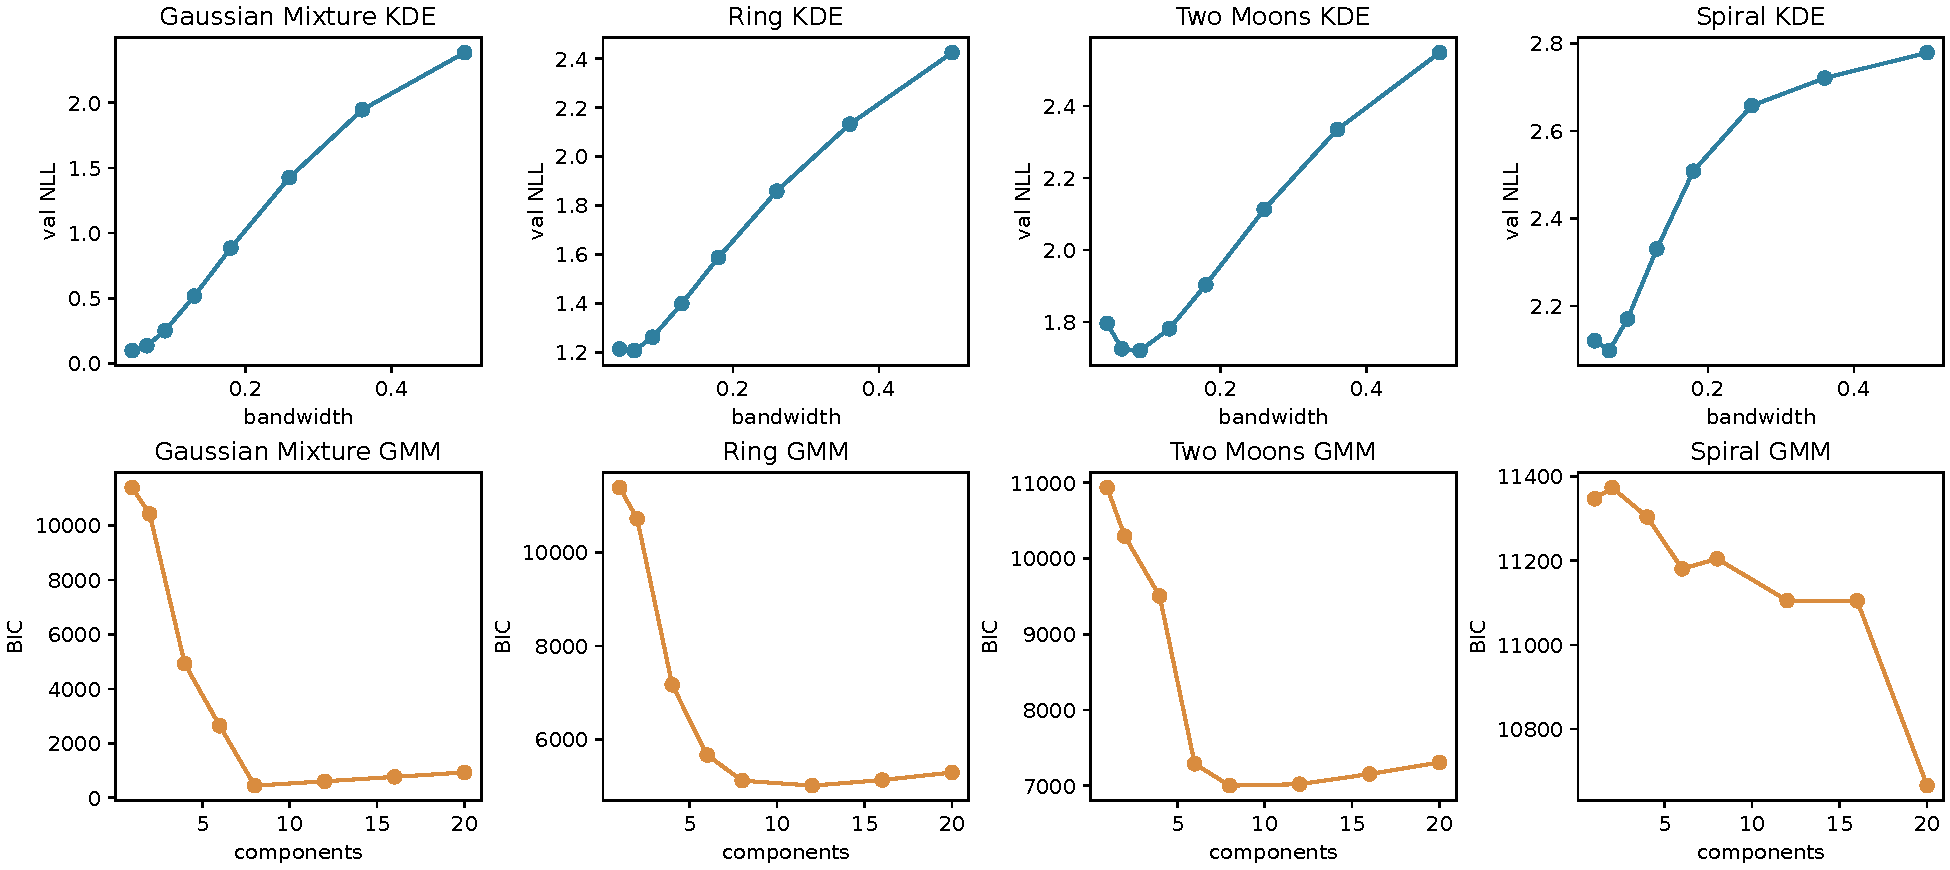
\includegraphics[width=\textwidth]{../results/figures/fig6_hyperparameter_sweep.pdf}
\caption{KDE 带宽和 GMM 组分数的扫描结果。KDE 使用验证 NLL 选带宽，GMM 使用 BIC 选组分数。}
\label{fig:sweep}
\end{figure}

图 \ref{fig:sweep} 展示了经典模型的关键超参数影响。KDE 带宽过小时会产生过多局部尖峰，带宽过大则会抹平 Ring 的中心空洞和 Spiral 的细节；GMM 组分数过少时无法拟合弯曲结构，组分数过多又会增加复杂度，因此 BIC 在拟合能力和复杂度之间做折中。

\subsection{异常点鲁棒性}

\begin{figure}[H]
\centering
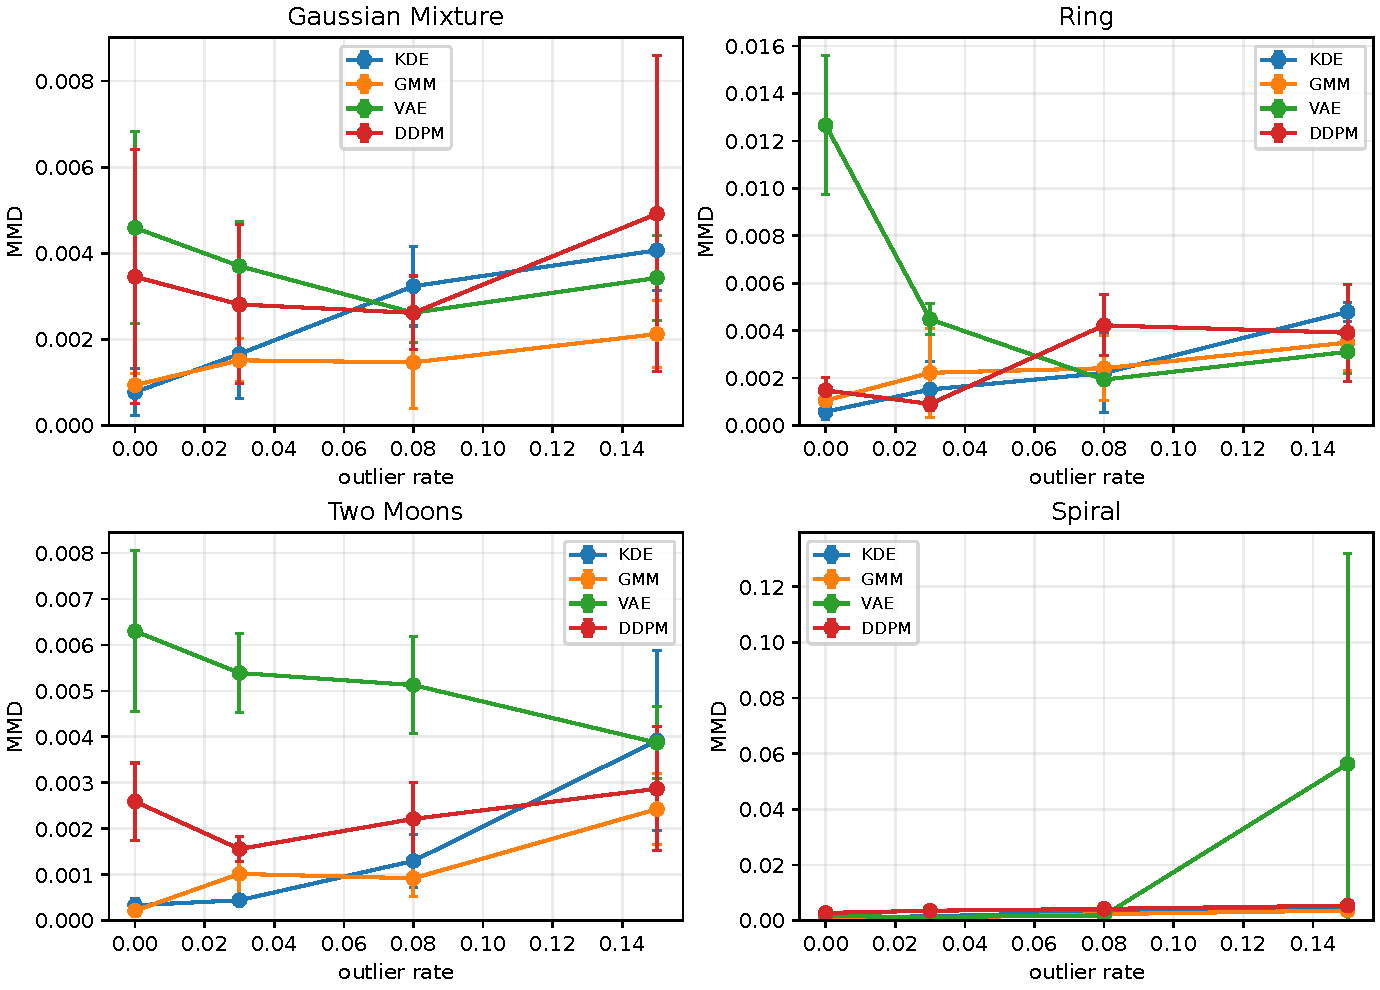
\includegraphics[width=0.88\textwidth]{../results/figures/fig8_robustness.pdf}
\caption{向训练集中加入不同比例均匀异常点后，四类模型的 MMD 变化。曲线为 3 个随机种子的均值，误差棒为标准差。}
\label{fig:robustness}
\end{figure}

异常点实验表明，四类模型都会受到训练污染影响，但影响方式不同。KDE 会在异常点附近放置核函数，从而抬高低密度区域的估计密度；GMM 可能分配额外成分解释异常点，导致有效组分被浪费；VAE 和 DDPM 则可能把异常点吸收到平滑生成分布中，表现为 Precision 或 MMD 的退化。由于鲁棒性实验也使用 3 个随机种子重复，图 \ref{fig:robustness} 的误差棒可以反映污染实验的不稳定性。这个结果说明，即使某个模型在干净数据上表现很好，也不能忽略训练数据质量对生成分布的影响。

\section{九、讨论与局限}

\subsection{为什么经典模型表现很强}

本实验中 KDE 和 GMM 的表现并不意外。本文使用的数据只有二维，训练样本达到每类 2000 个，且测试分布和训练分布来自同一官方生成机制。此时非参数估计和混合高斯都有足够数据覆盖支撑区域。尤其是 KDE，它没有强加有限高斯成分假设，只需通过带宽控制局部平滑，因此在 Ring、Two Moons 和 Spiral 这类弯曲支撑上也能保持很高 Coverage。相比之下，VAE 和 DDPM 的神经网络结构需要通过优化学习密度形状，在这种低维合成任务上不一定比直接利用样本邻域更有效。因此，本文结论应理解为“在当前二维设置下经典模型是强基线”，而不是“经典模型普遍优于神经生成模型”。

\subsection{VAE 的过平滑现象}

VAE 在四类数据上 Precision 明显偏低，说明生成样本常落在真实支撑之外。原因在于标准正态潜空间和均方重构误差倾向于学习连续平滑映射。当真实分布具有空洞或窄流形时，VAE 容易在流形之间插值，产生视觉上“填充空白”的样本。这个现象在 Ring 和 Two Moons 上最明显。

\subsection{DDPM 的表达能力与成本}

DDPM 长训练后可以生成可辨认的 Ring、Two Moons 和 Spiral 结构，说明逐步去噪模型确实具备表达复杂非线性几何的能力。但它仍需要更长训练和多步采样，训练时间约为 KDE 的十倍以上；在当前二维数据上，其 MMD、SWD 和 Precision 并没有压过 KDE。对本课程作业而言，DDPM 的价值更多在于展示现代生成模型思想、条件生成扩展和复杂几何表达能力，而不是在所有指标上取得最优。

\subsection{局限性}

本文仍有若干局限：
\begin{enumerate}
    \item 数据来自题目提供的二维合成生成器，结论严格对应该官方生成机制，不能外推到真实高维数据；
    \item VAE 和 DDPM 没有做大规模超参数搜索，因此神经模型可能不是最优实现；
    \item 本文没有实现 RealNVP 等精确似然神经模型，NLL 比较只覆盖 KDE 和 GMM；
    \item Precision/Coverage 的半径选择依赖近邻距离，改变半径会影响绝对数值；二维网格支撑覆盖率也受网格分辨率影响；
    \item 二维合成任务不能直接说明高维图像生成中的模型优劣。
\end{enumerate}

\section{十、结论}

本文完成了二维分布生成建模任务，并比较了 KDE、GMM、VAE 和 DDPM 四类模型。主要结论如下：
\begin{enumerate}
    \item 在官方二维生成器和每类 2000 个训练样本设置下，KDE 是最强整体基线，在四类分布上均取得最低 MMD、最低 SWD 和最高 Coverage；
    \item Gaussian Mixture 上 GMM 的 NLL 和 Precision 最好，但 KDE 的样本分布距离更低，说明密度拟合和样本匹配并不完全等价；
    \item Ring 和 Two Moons 上 KDE 表现最好，说明局部核平滑能自然保持闭合或弯曲支撑；
    \item Spiral 上 KDE 仍取得最低 MMD，GMM 与 DDPM 接近但 Precision 较低，体现出长曲线支撑对局部贴合的要求；
    \item VAE 在本设置中明显过平滑，生成样本容易进入低密度区域；
    \item 条件 DDPM 可以用一个模型按标签生成四类分布，但共享参数会带来一定性能损失；
    \item 多个评价指标会给出不同侧面的结论，因此生成模型评价必须结合可视化、MMD/SWD、Precision/Coverage、支撑覆盖率和 NLL。
\end{enumerate}

如果继续改进，最有价值的方向是加入 RealNVP 或 Neural Spline Flow 作为精确似然神经模型。这样可以在保持神经模型表达能力的同时，对 NLL 做更公平的横向比较，也能检验神经生成模型是否能在二维官方数据上同时取得好样本距离和好似然。

\clearpage
\section{十一、复现实验、分工与 AI 使用说明}

\subsection{复现实验}

在项目根目录运行：
\begin{verbatim}
python final_project/distribution2d_gen/generate_data.py \
  --output-dir final_project/data --plot

MPLCONFIGDIR=/tmp/mplconfig XDG_CACHE_HOME=/tmp \
python final_project/src/run_experiments.py \
  --out-dir final_project/results \
  --n-train 2000 --n-test 2000 --n-generate 2000 \
  --seeds 0 1 2 --vae-epochs 320 --ddpm-epochs 2500 --ddpm-steps 100
\end{verbatim}

本次运行环境如下：Python 3.12.7，NumPy 1.26.4，SciPy 1.13.1，scikit-learn 1.5.1，PyTorch 2.5.1，Matplotlib 3.9.2，macOS 15.3.1，CPU 运行。完整记录见运行清单：
\url{final_project/results/run_manifest.json}。

\subsection{文件清单}

\begin{longtable}{p{0.48\textwidth}p{0.42\textwidth}}
\toprule
文件或目录 & 说明 \\
\midrule
\texttt{distribution2d\_gen/generate\_data.py} & 题目提供的二维分布数据生成代码 \\
\texttt{data/} & 官方生成器默认 seed 生成的 train/test/hidden 数据文件 \\
\texttt{src/run\_experiments.py} & 数据生成、模型训练、评价与绘图脚本 \\
\texttt{results/metrics\_summary.csv} & 聚合指标表 \\
\texttt{results/metrics\_by\_seed.json} & 逐 seed 完整指标 \\
\texttt{results/conditional\_metrics\_summary.csv} & 条件 DDPM 聚合指标 \\
\texttt{results/robustness.csv} & 多模型异常点鲁棒性指标 \\
\texttt{results/figures/} & 报告使用的 PDF/PNG 图像 \\
\texttt{results/tables/} & LaTeX 表格片段 \\
\texttt{report/main.tex} & 本报告源码 \\
\texttt{report/main.pdf} & 编译后的报告 PDF \\
\bottomrule
\end{longtable}

\subsection{分工情况}

本次作业为独立完成。分工记录如下：模型方案设计、代码实现、实验运行、图表制作、论文撰写、结果核验和最终排版均由孙悦淳完成。

\subsection{AI 使用说明}

AI 工具用于辅助规划报告结构、整理实验代码、检查叙事逻辑和排版细节。所有实验数据、指标数值和图像均由本地脚本实际运行生成，未手工编造。最终结论根据 \texttt{metrics\_summary.csv}、图像文件和运行清单核对后写入报告。

\appendix
\section{附录 A：关键实现片段}

以下片段展示了 MMD 的核心计算逻辑：
\begin{verbatim}
def mmd_rbf(x, y):
    z = np.vstack([x, y])
    sample = z[rng.choice(len(z), size=min(600, len(z)), replace=False)]
    sigma2 = np.median(pairwise_sq_dists(sample, sample))
    kxx = np.exp(-pairwise_sq_dists(x, x) / (2 * sigma2)).mean()
    kyy = np.exp(-pairwise_sq_dists(y, y) / (2 * sigma2)).mean()
    kxy = np.exp(-pairwise_sq_dists(x, y) / (2 * sigma2)).mean()
    return max(kxx + kyy - 2 * kxy, 0.0)
\end{verbatim}

\section{附录 B：结论验证表}

\begin{table}[H]
\centering
\caption{主要结论与证据对应关系}
\resizebox{\textwidth}{!}{
\begin{tabular}{lll}
\toprule
结论 & 证据 & 判定 \\
\midrule
KDE 是官方二维数据上的强整体基线 & KDE 在四类数据集 MMD/SWD/Coverage 均最佳 & 支持 \\
VAE 存在过平滑 & Ring/Two Moons 可视化和低 Precision & 支持 \\
DDPM 可表达弯曲结构但局部仍不稳 & 可视化可见环、月牙、螺旋形态，但 Precision/SWD 低于 KDE & 支持 \\
条件生成可行但有性能代价 & 条件 DDPM 可生成四类分布但部分 MMD 高于独立模型 & 支持 \\
单一指标不足 & MMD、Coverage、Precision 排名不完全一致 & 支持 \\
异常点会影响生成质量 & 四类模型 Robustness 曲线随 outlier rate 变化 & 支持 \\
\bottomrule
\end{tabular}
}
\end{table}

\begin{thebibliography}{99}
\bibitem{kingma2014vae}
D. P. Kingma and M. Welling.
Auto-Encoding Variational Bayes.
International Conference on Learning Representations, 2014.

\bibitem{sohl2015diffusion}
J. Sohl-Dickstein, E. Weiss, N. Maheswaranathan, and S. Ganguli.
Deep Unsupervised Learning using Nonequilibrium Thermodynamics.
International Conference on Machine Learning, 2015.

\bibitem{ho2020ddpm}
J. Ho, A. Jain, and P. Abbeel.
Denoising Diffusion Probabilistic Models.
Advances in Neural Information Processing Systems, 2020.

\bibitem{dinh2017realnvp}
L. Dinh, J. Sohl-Dickstein, and S. Bengio.
Density Estimation using Real NVP.
International Conference on Learning Representations, 2017.

\bibitem{gretton2012mmd}
A. Gretton, K. M. Borgwardt, M. J. Rasch, B. Scholkopf, and A. Smola.
A Kernel Two-Sample Test.
Journal of Machine Learning Research, 2012.

\bibitem{arjovsky2017wgan}
M. Arjovsky, S. Chintala, and L. Bottou.
Wasserstein Generative Adversarial Networks.
International Conference on Machine Learning, 2017.

\bibitem{kynkaanniemi2019precision}
T. Kynkaanniemi, T. Karras, S. Laine, J. Lehtinen, and T. Aila.
Improved Precision and Recall Metric for Assessing Generative Models.
Advances in Neural Information Processing Systems, 2019.

\bibitem{sklearnkde}
scikit-learn developers.
Density Estimation and Gaussian Mixture Models User Guide.
\url{https://scikit-learn.org/stable/modules/density.html},
\url{https://scikit-learn.org/stable/modules/mixture.html}.
\end{thebibliography}

\end{document}
